\documentclass{ctexart}

\usepackage{amsmath}

\usepackage{amsthm}

\usepackage{amssymb}

\usepackage{bm}

\usepackage{graphicx}

\usepackage{listings}
\lstset{
basicstyle=\scriptsize
}

\usepackage{caption}

\begin{titlepage}

\title{微分方程数值解 \\ 第七周作业}

\author{于慧倩 \\ 14300180118}

\date{2017年4月}

\end{titlepage}

\begin{document}

\maketitle

\newpage

\begin{enumerate}
%第一题
\item
用Newton表示重新写出Adams格式。

\[ u_{n+1}-u_n = \int_{t_n}^{t_{n+1}} f(t)dt =  \left\{ \begin{array}{rl}\int_0^1 f(t_n+s \Delta t) \mbox{d}s \mbox{d} t  &(\mbox{显式}) \\
 \int_0^1 f(t_{n+1} - \alpha \Delta t) \mbox{d}s \mbox{d} t &(\mbox{隐式})\end{array} \right.\]

首先对于显式:
\[f(t_n+s \Delta t)=\bigtriangledown f_n+\frac{\bigtriangledown f_n}{\Delta t}s \Delta t+\frac{\bigtriangledown^2 f_n}{2!(\Delta t)^2}(s\Delta t)((s+1)\Delta t)+\dots\]

由于
\[ \frac{s(s-1)(s-2)\dots(s-j+1)}{j!}={s\choose j}\]
所以有
\[f(t_n+s\Delta t) =\sum_{j=0}^{k}(-1)^j {-s\choose j}  \bigtriangledown^j f_n \]

故有
\[u_{n+1}-u_n =\sum_{j=0}^k (-1)^j \int_0^1 {-s\choose j}\bigtriangledown^j f_n \mbox{d}s \mbox{d}t\]

对于隐式:
\[ f(t_{n+1} - \alpha \Delta t) =\bigtriangledown f_{n+1} + \frac{\bigtriangledown^1 f_{n+1}}{\Delta}(- \alpha)\Delta t+\frac{\bigtriangledown^2 f_{n+1}}{\Delta t^2 2!}(-\alpha)(1-\alpha)\Delta t+\dots\]

由于
\[ \frac{(\alpha)(\alpha+1)(\alpha+2)\dots(\alpha+j-1)}{j!}={\alpha\choose j}\]
故有
\[ u_{n+1}-u_n = \sum_{j=0}^k (-1)^j \int_0^1 {\alpha\choose j}\bigtriangledown^j f_{n+1} \mbox{d}s \mbox{d}t \]


\item P118 1

\begin{enumerate}

\item 写出精确的\(u(t)\)的表达式

\[u(t)=e^{\lambda t}(u_0+\frac{\lambda}{\lambda^2+1} (e^{\lambda t} \sin t+\lambda e^{\lambda t}\cos t-\lambda)) \]

\item 对\(\lambda =1,10,100,1000\),分别用显式Euler格式和隐式Euler格式求解:

当\(\Delta t = 10^{-4}\)时,显式Euler方法与隐式Euler方法都能较准确的计算出函数值。

\begin{enumerate}

\item \(u_0=0\)时,显式Euler格式画图如下:

\centerline{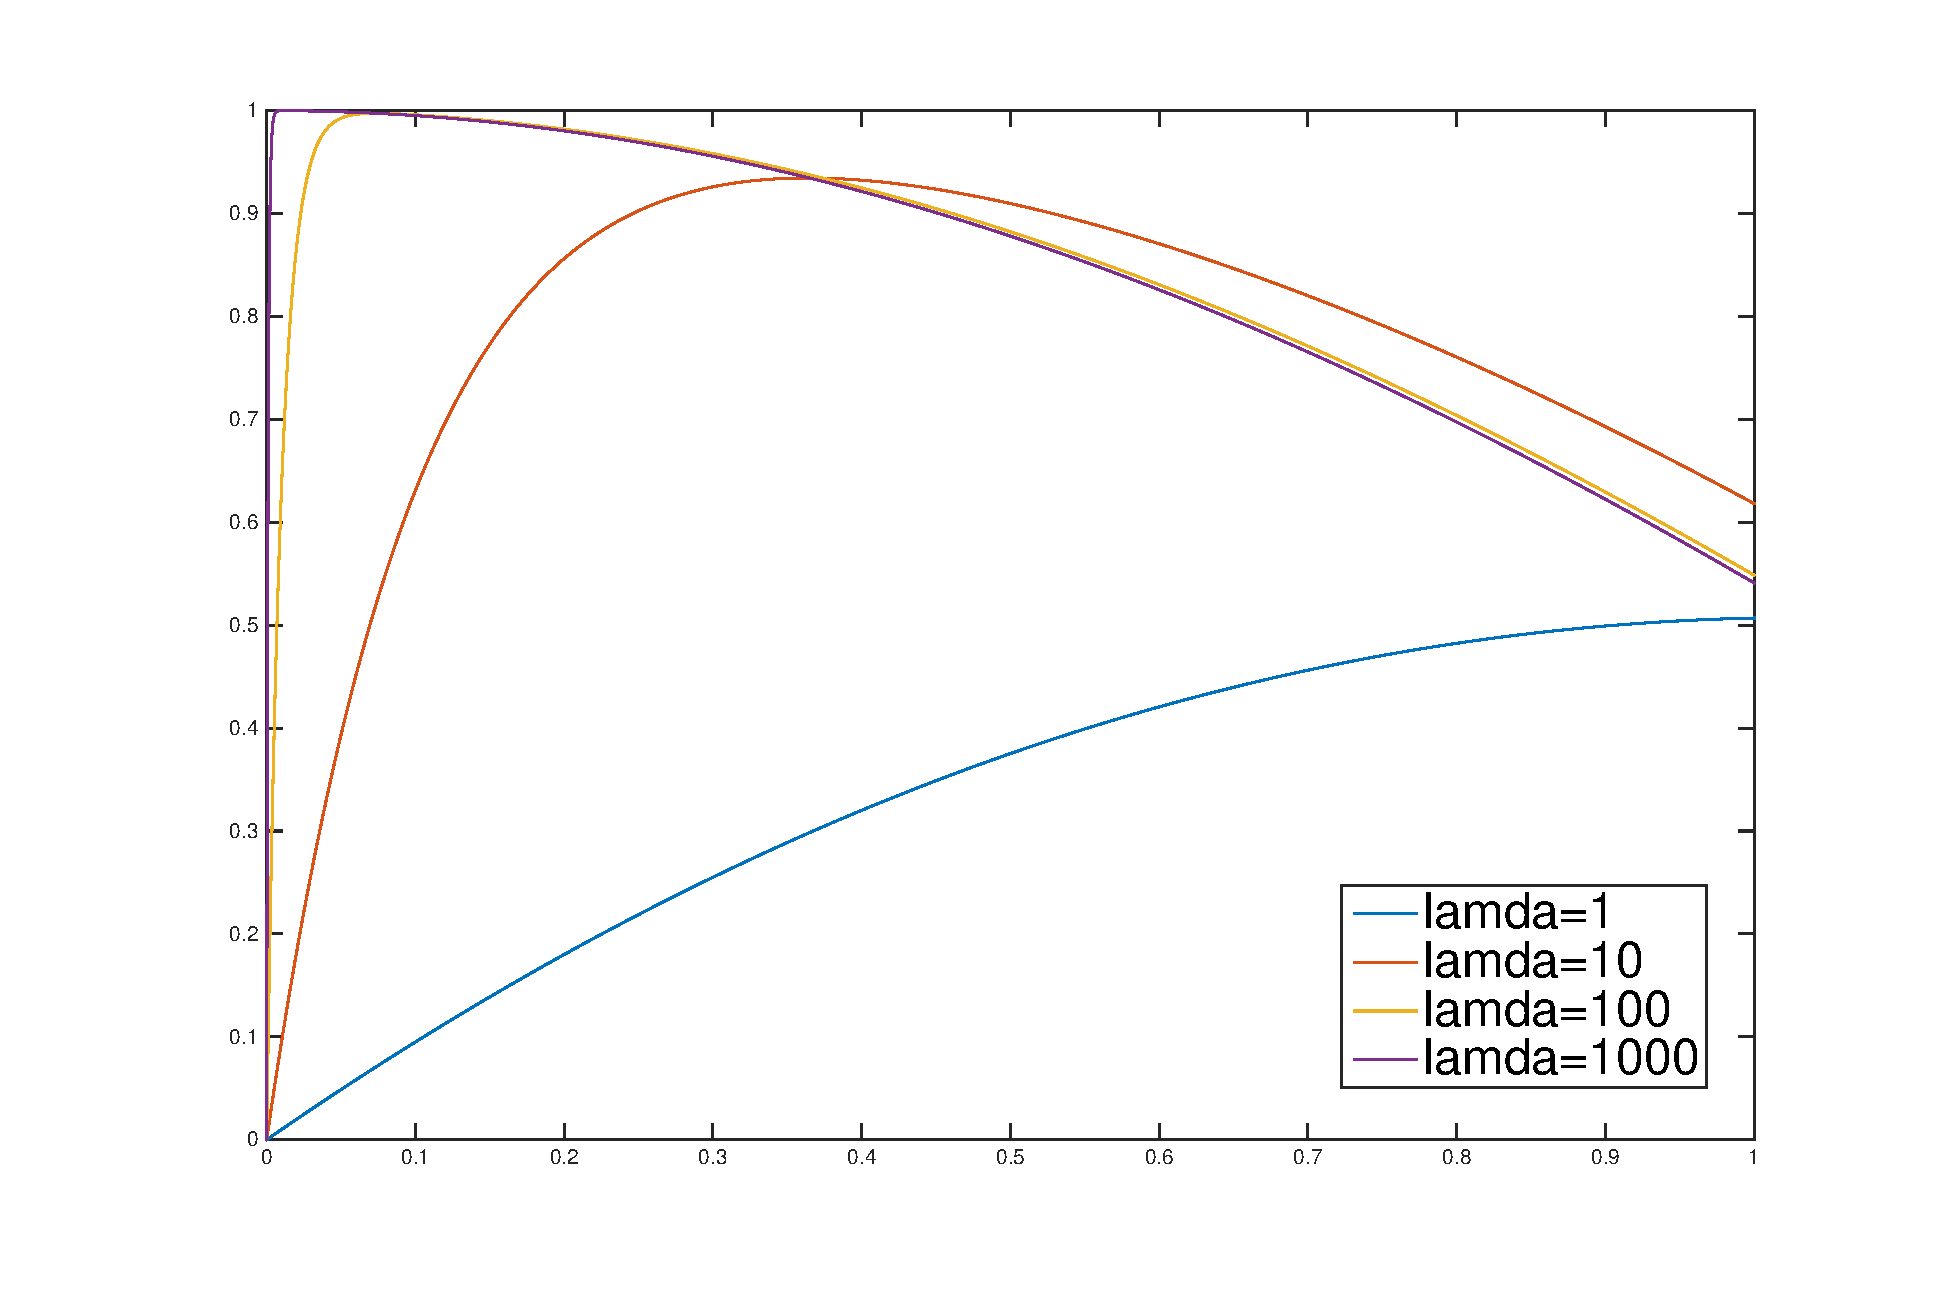
\includegraphics[width=5.5in]{X0.eps}}

\item \(u_0=1\)时,显式Euler格式画图如下:

\centerline{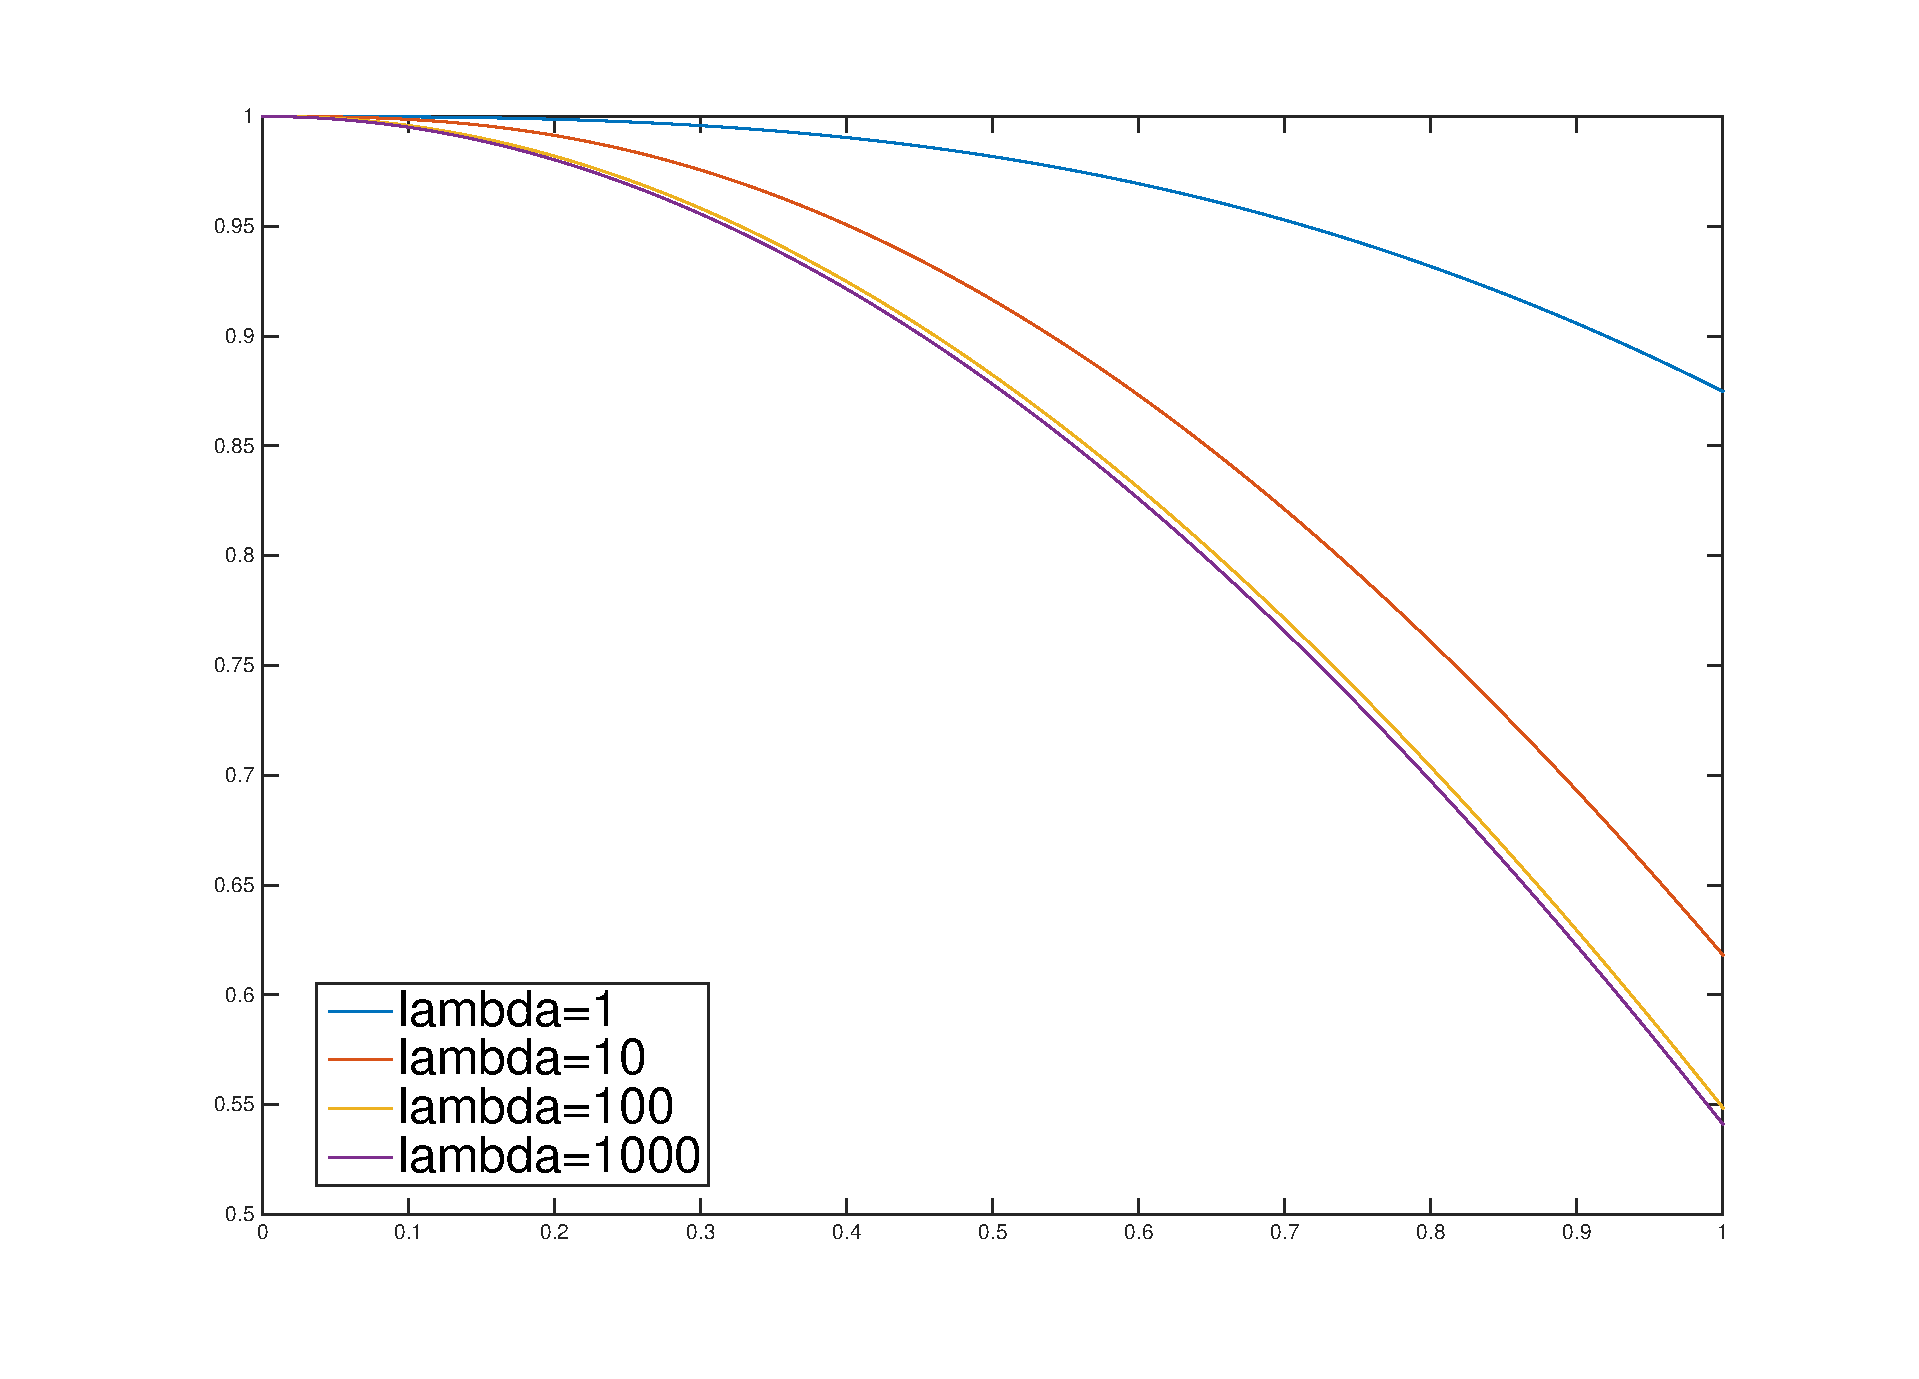
\includegraphics[width=5.5in]{2_1.eps}}
\centerline{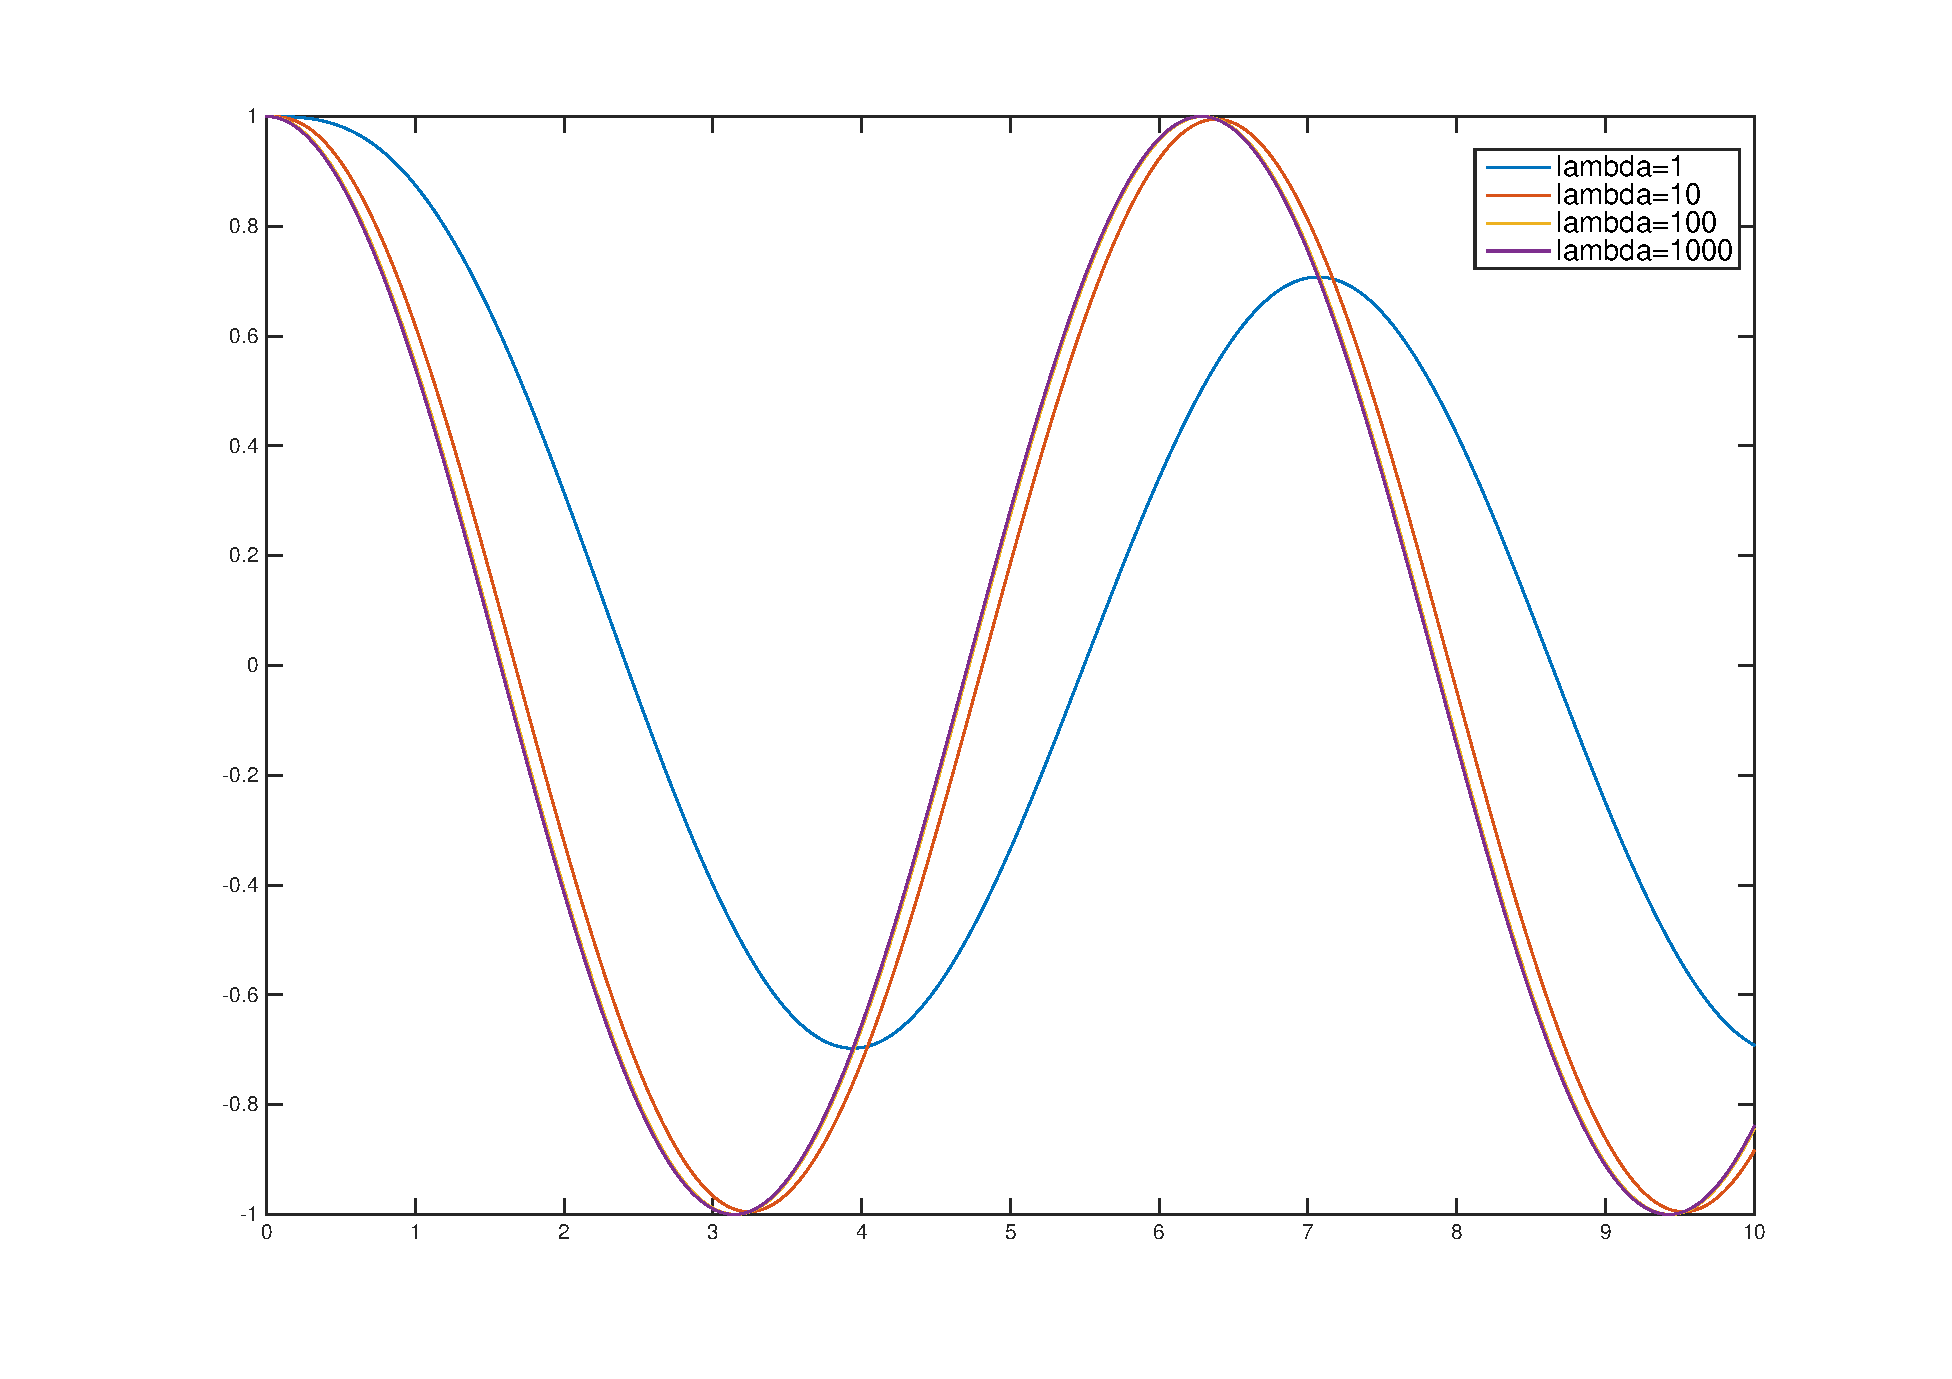
\includegraphics[width=5.5in]{2_2.eps}}

\item \(u_0=0\)时,显式Euler格式画图如下:

\centerline{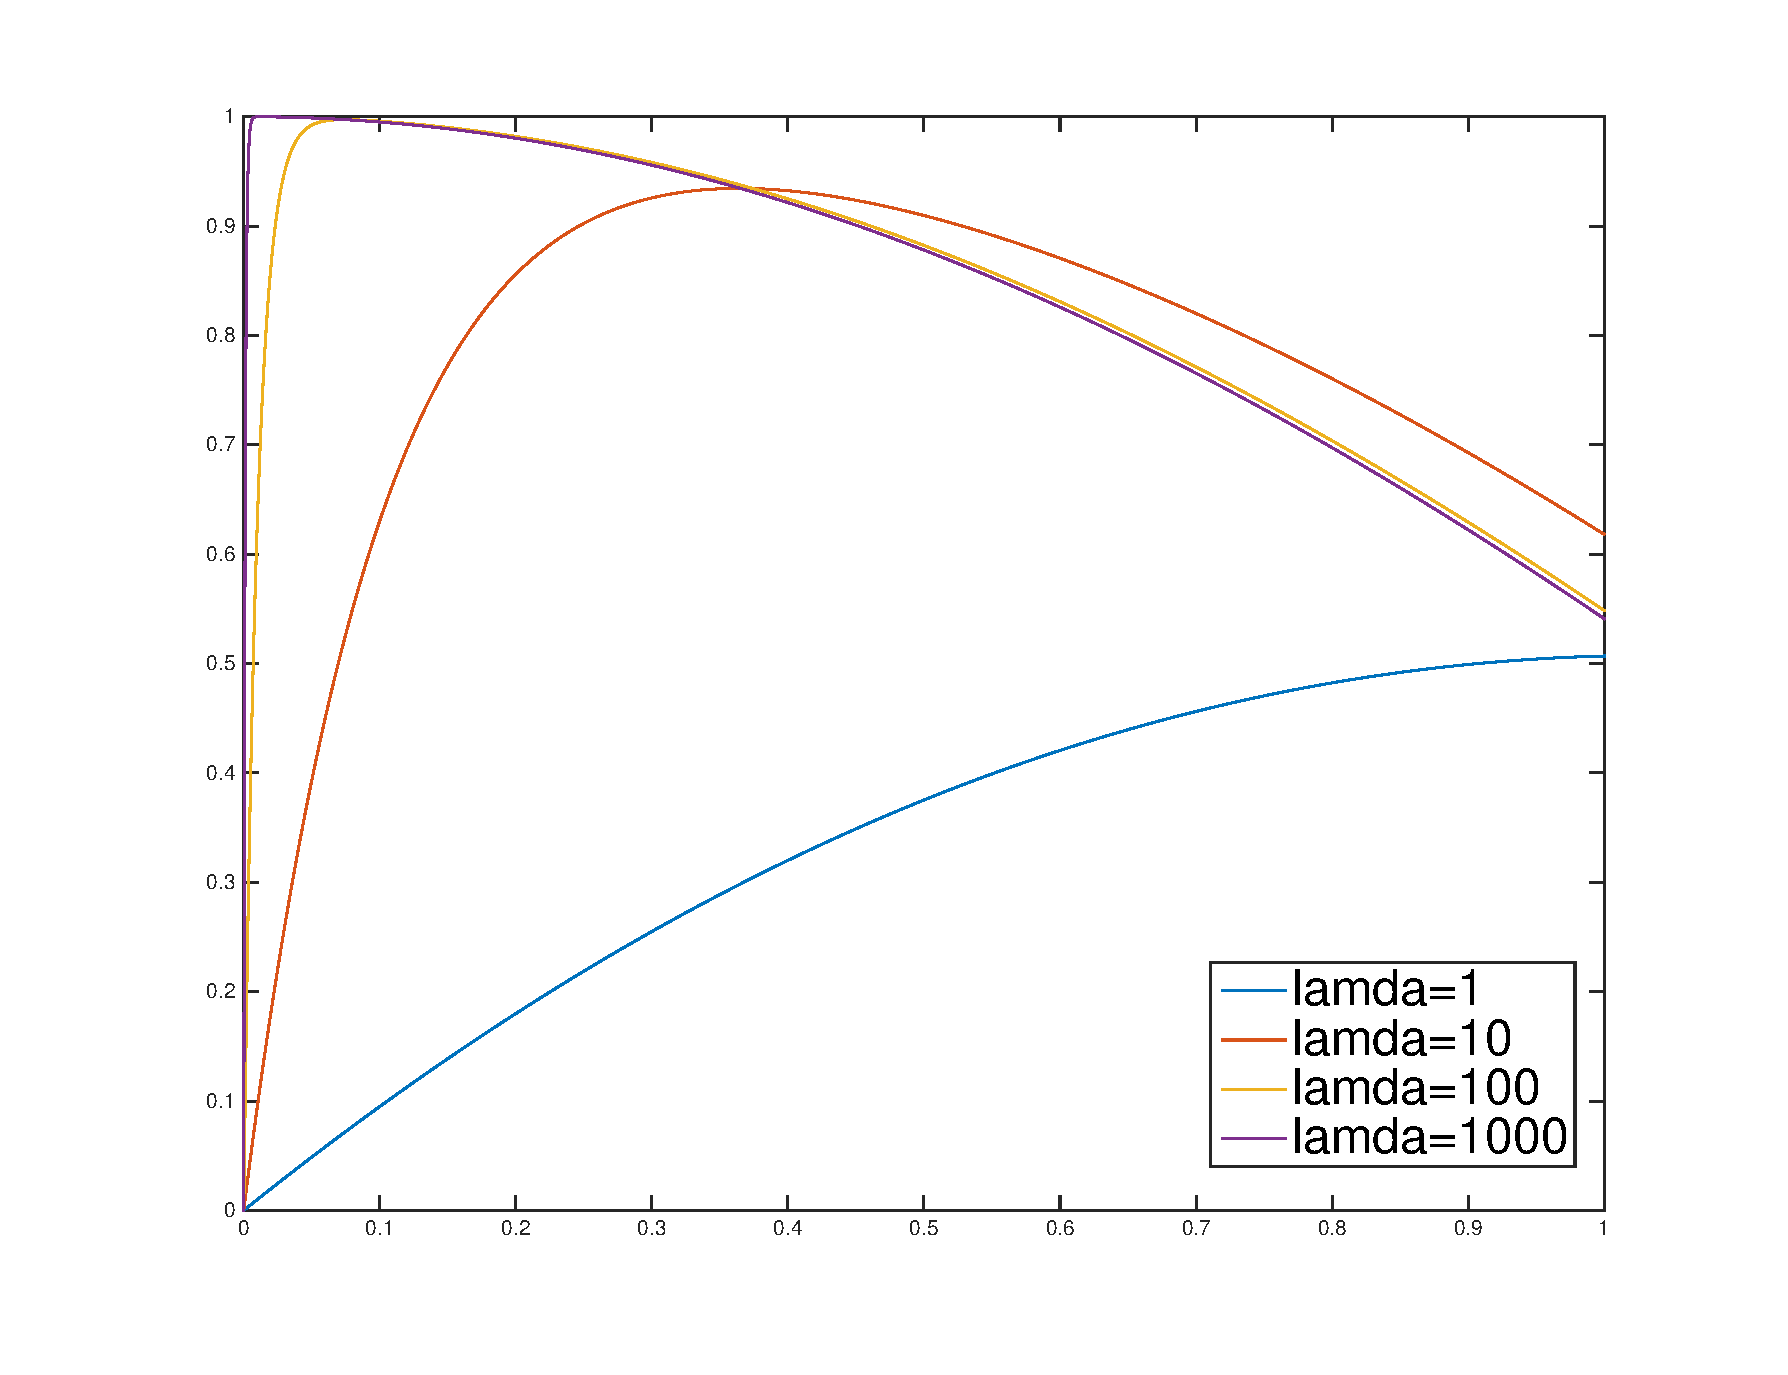
\includegraphics[width=5.5in]{Y0.eps}}

\item \(u_0=1\)时,隐式Euler格式画图如下

\centerline{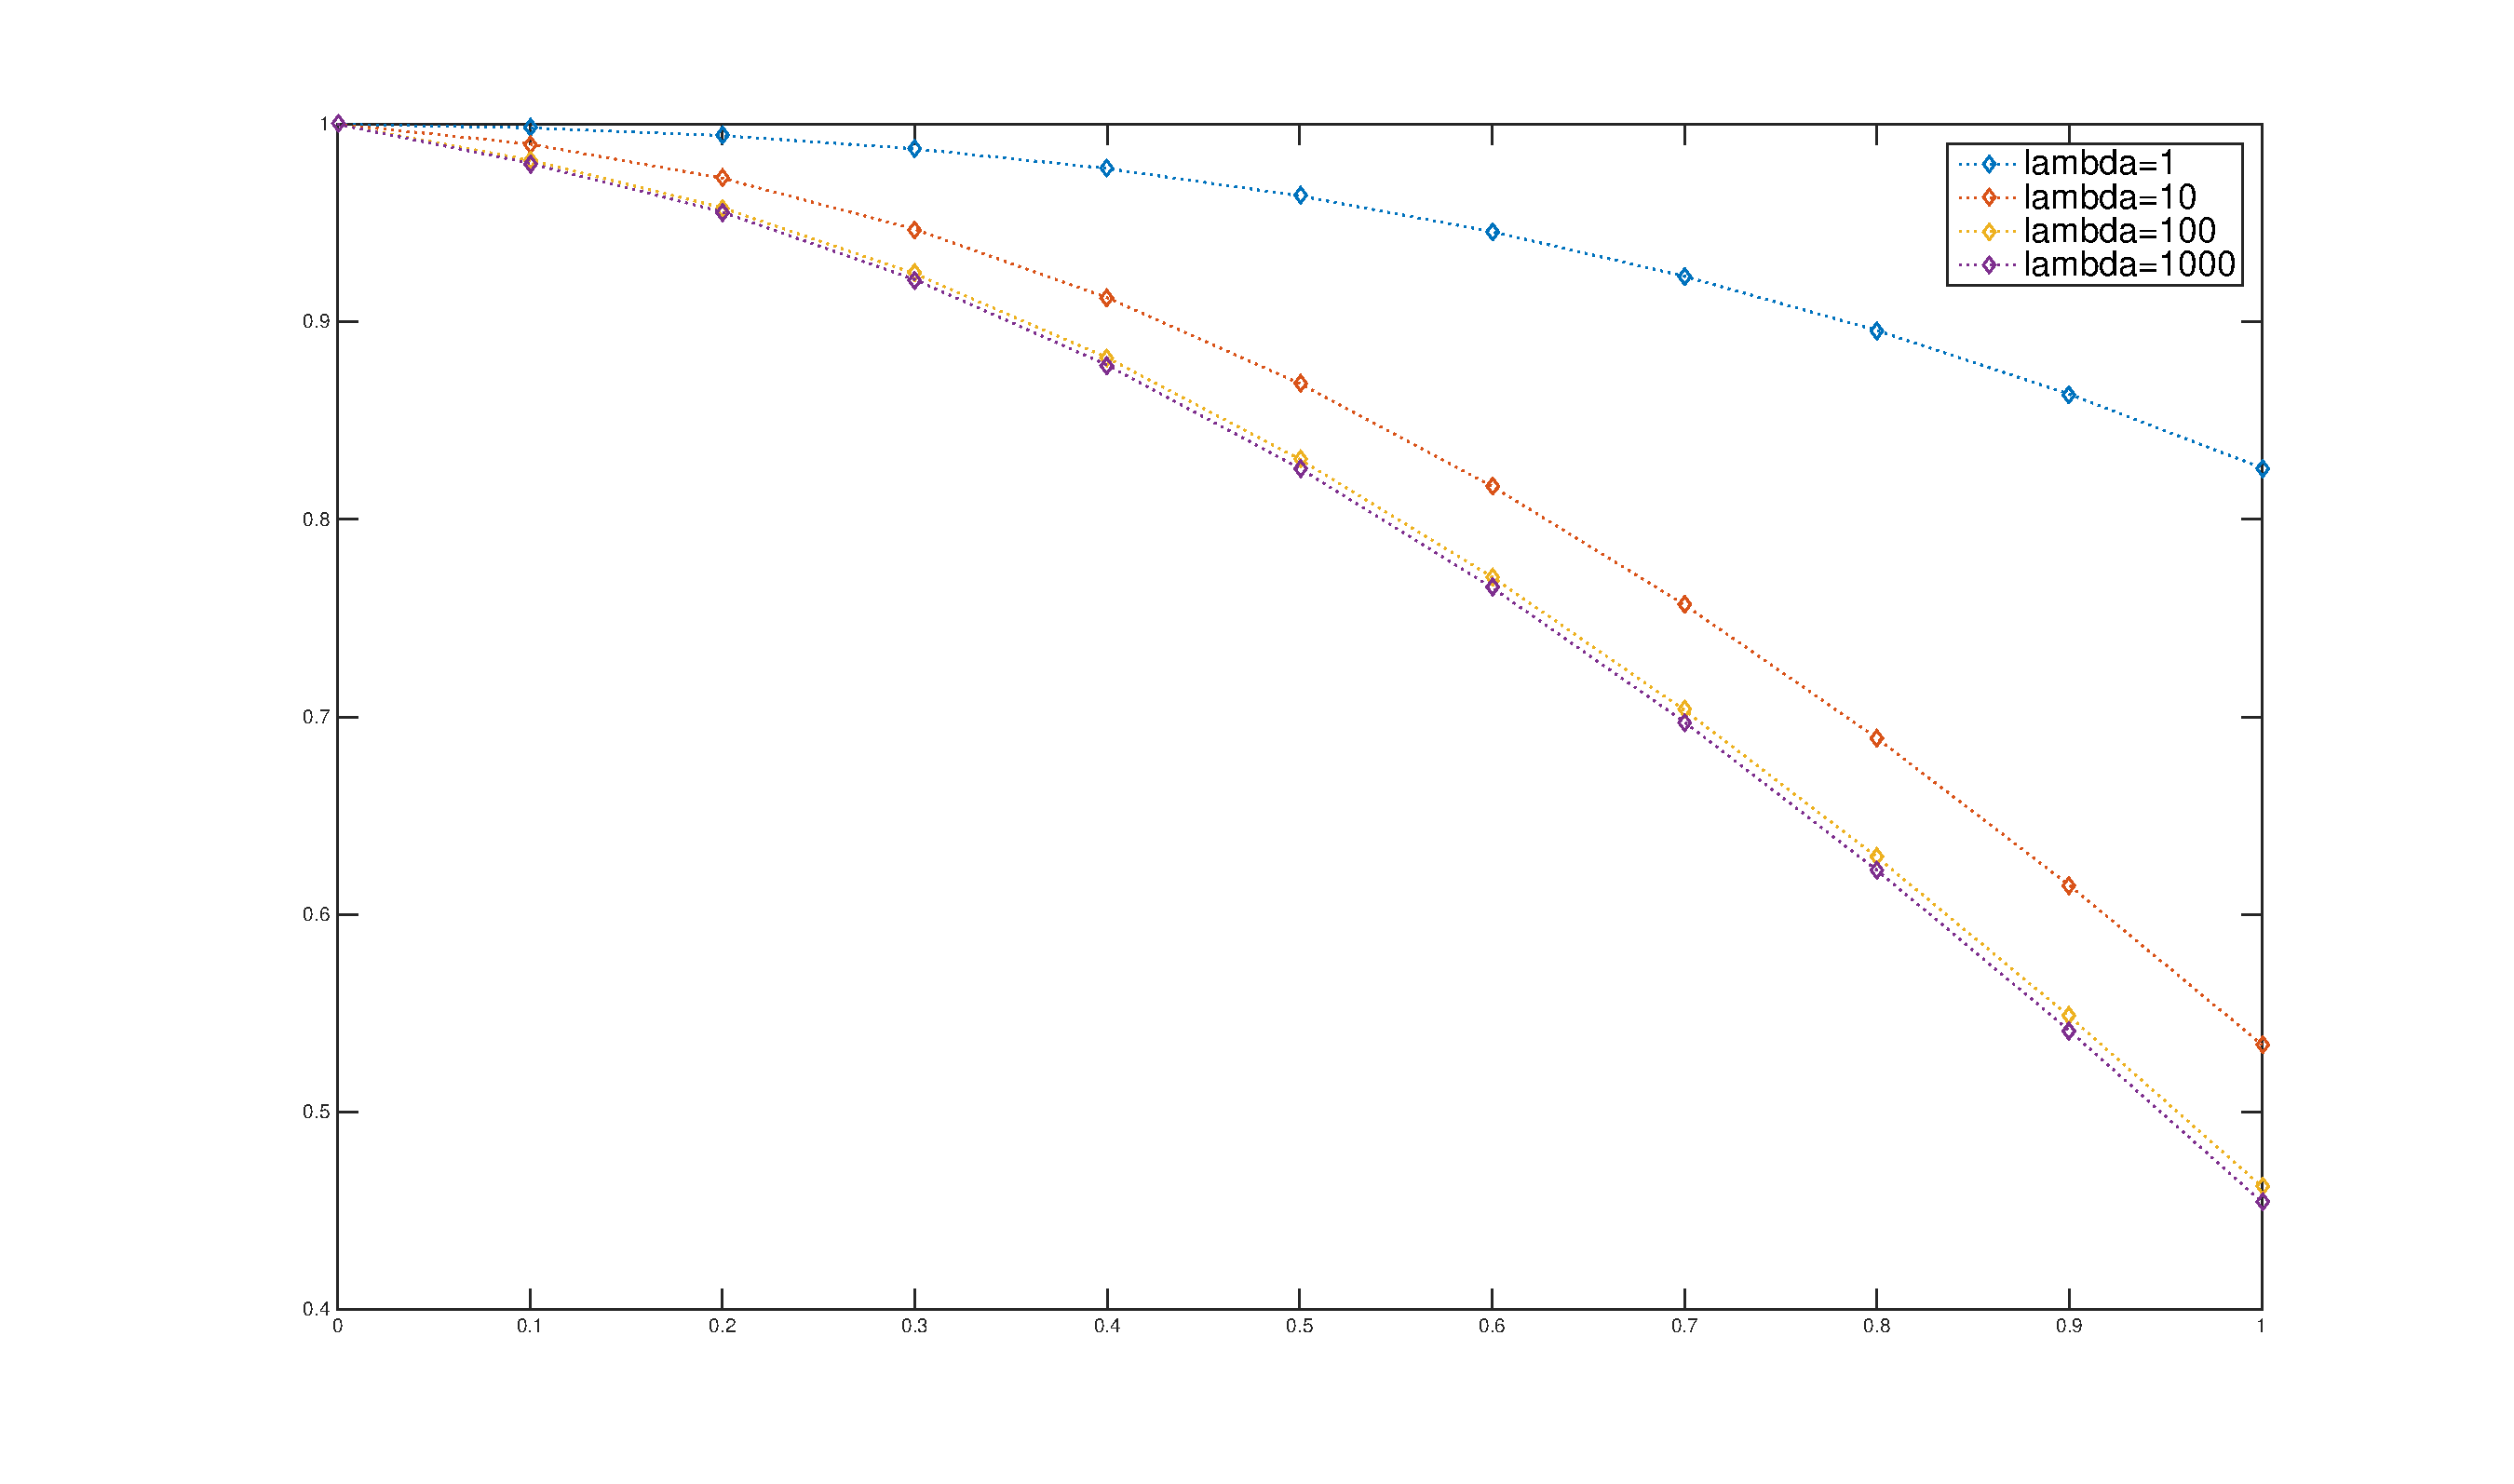
\includegraphics[width=5.5in]{2_4.eps}}
\centerline{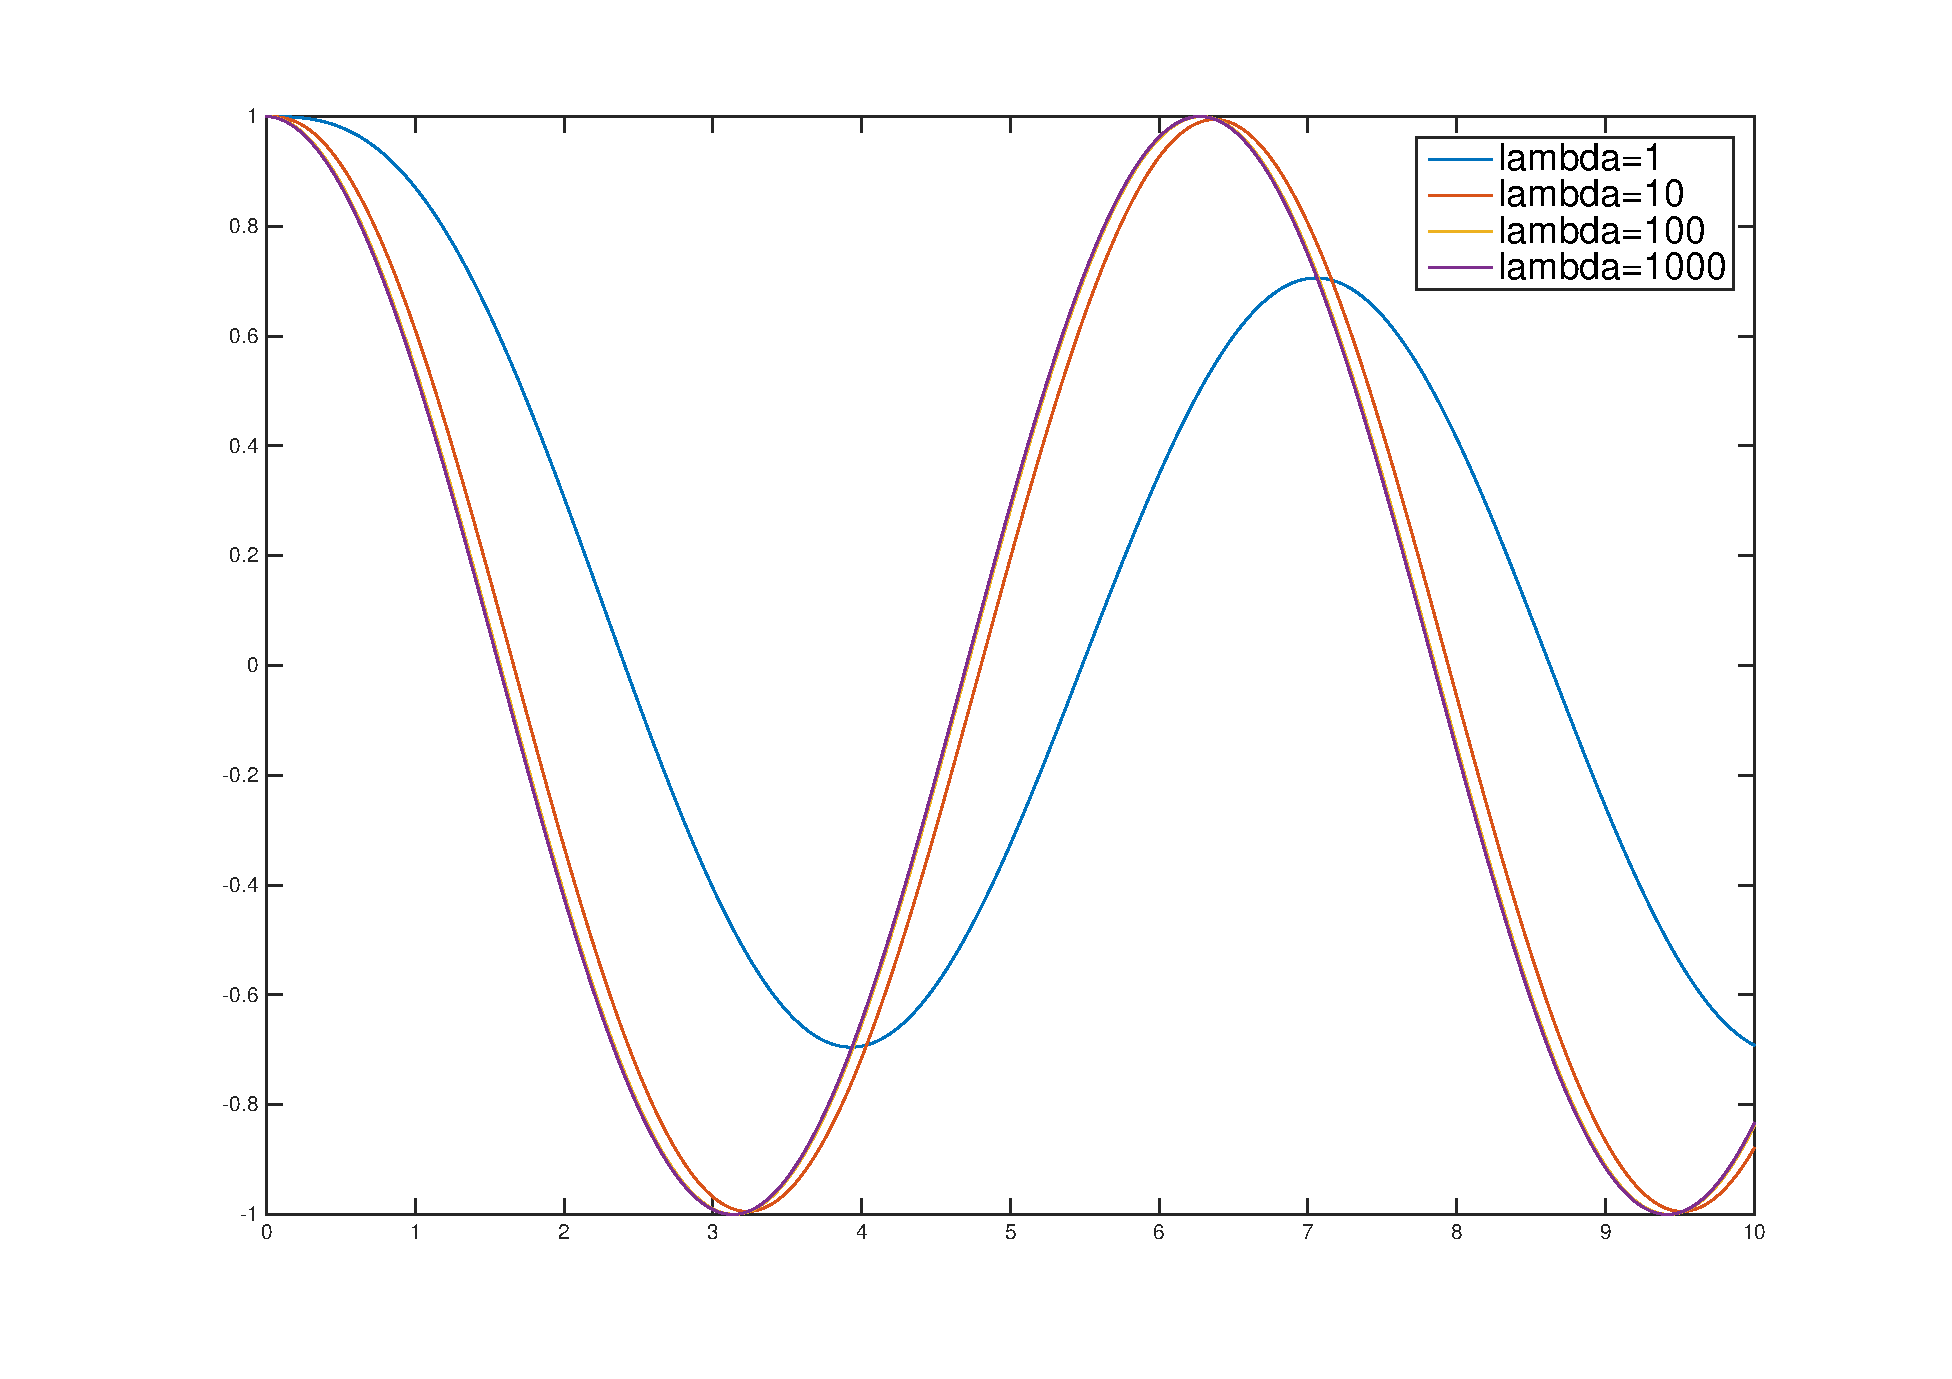
\includegraphics[width=5.5in]{2_3.eps}}
\end{enumerate}


当\(\Delta t = 10^{-2}\)时,显式Euler方法无法计算\(\lambda\)较大时的结果。

\begin{enumerate}

\item  \(u_0=0\)

\centerline{\includegraphics[width=5.5in]{X011.eps}}

\item  \(u_0=1\)

\centerline{\includegraphics[width=5.5in]{X01.eps}}

\end{enumerate}


\item 比较用Adams方法和Gear方法,计算\(\lambda=1000\)时的数值行为。

当\(\Delta t = 10^{-4}\)时,Adamas方法(初值用精确值代表)与Gear方法都能较准确的计算出函数值。

\begin{enumerate}
\item  \(u_0=0\)时,Adams方法如图

\centerline{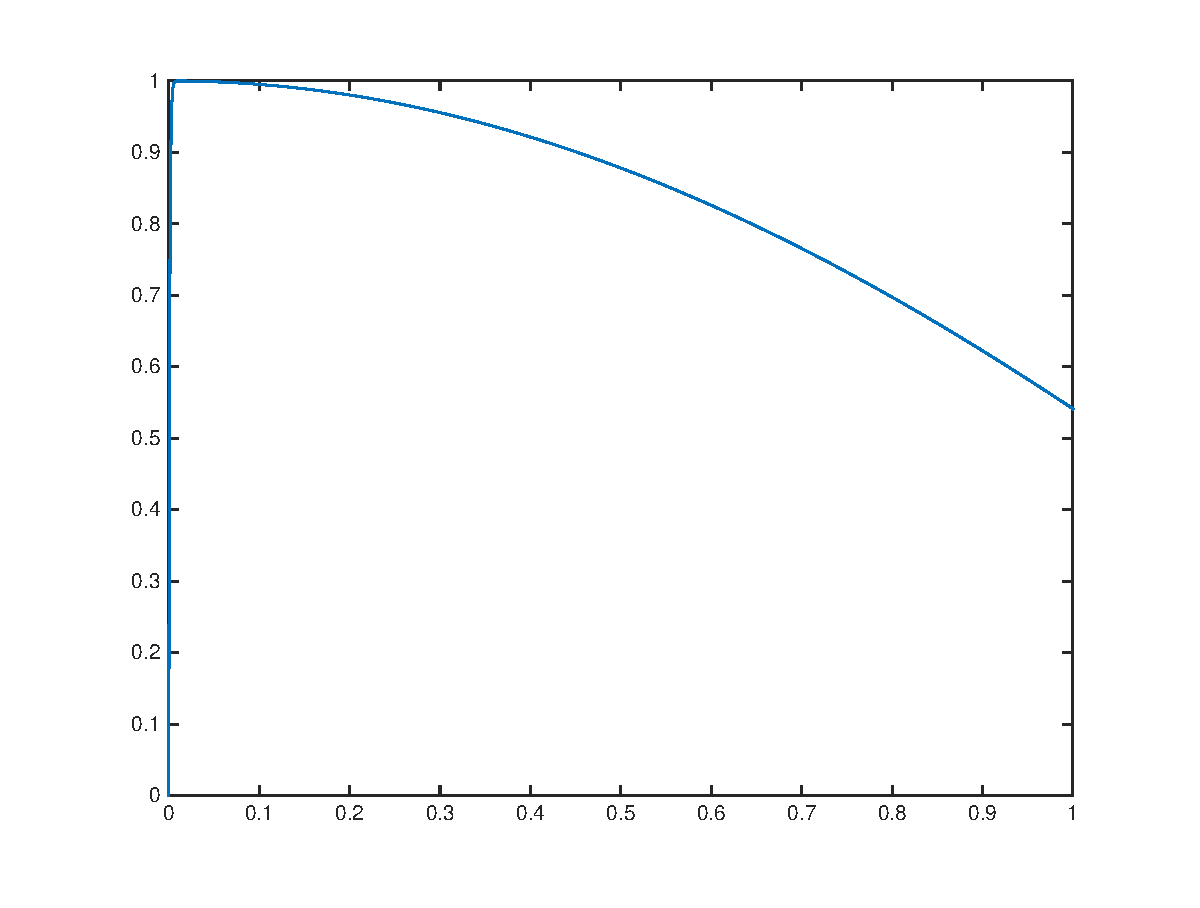
\includegraphics[width=5.5in]{Adams0.eps}}

\item  \(u_0=1\)时,Adams方法如图

\centerline{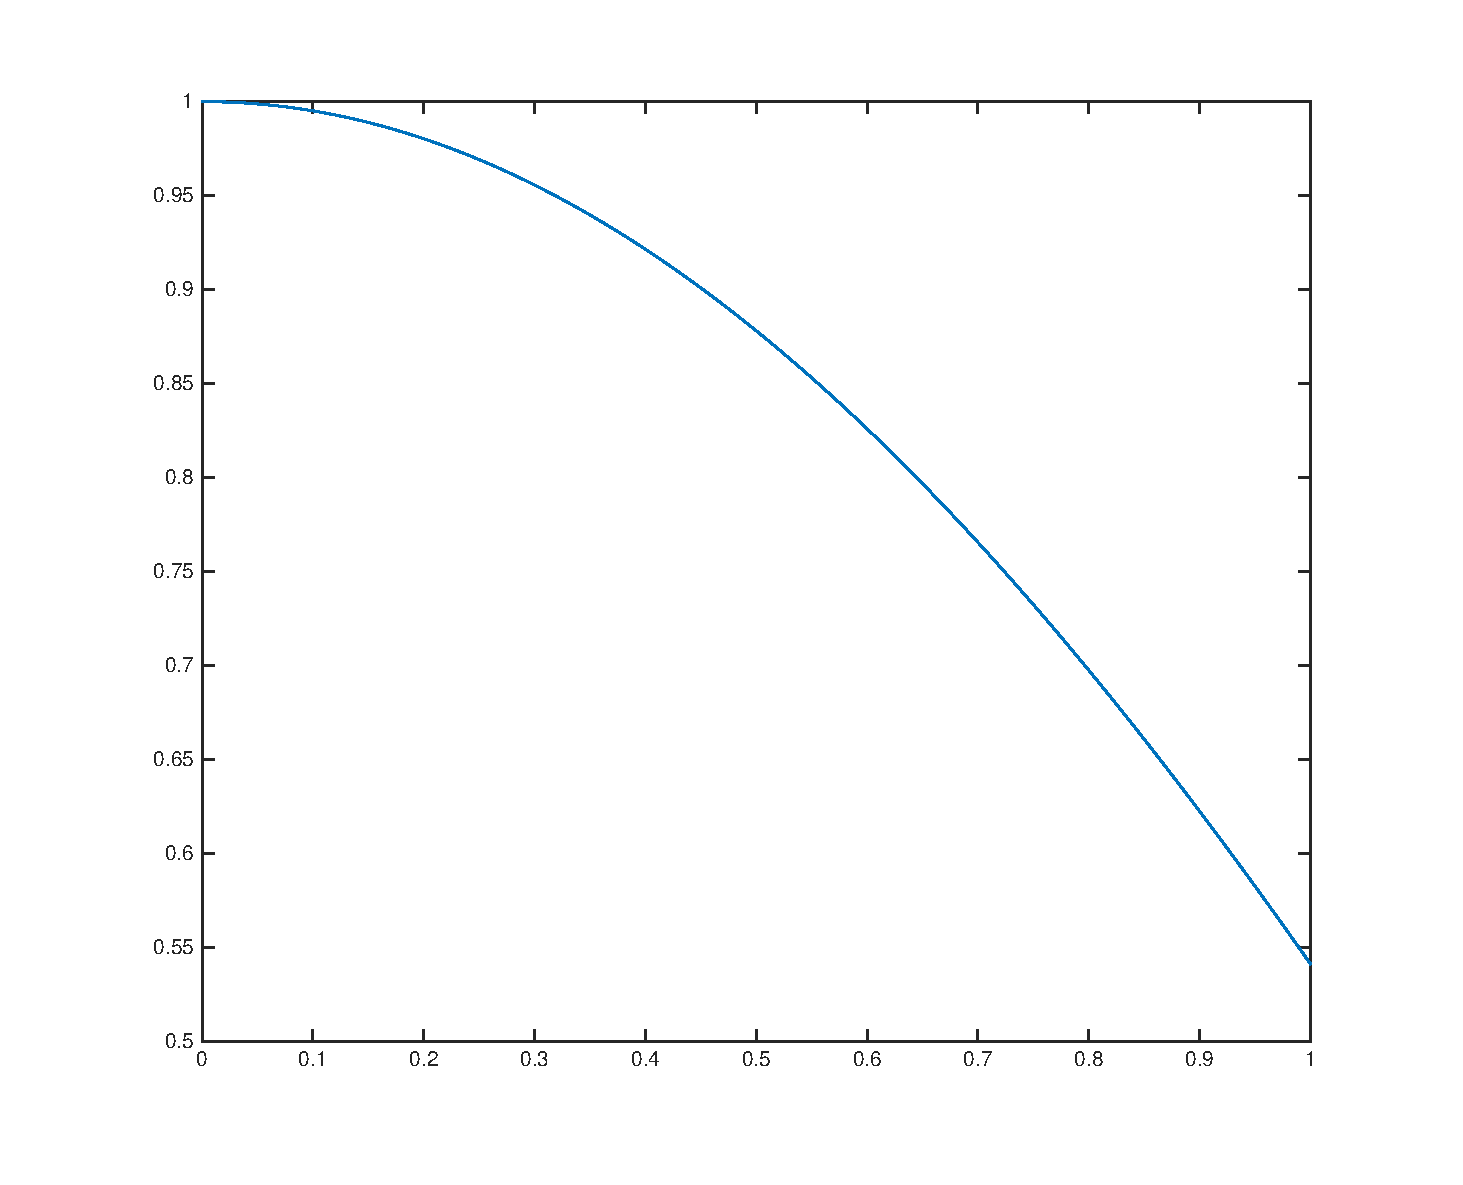
\includegraphics[width=5.5in]{Adams1.eps}}

\item  \(u_0=0\)时,Gear方法如图


\centerline{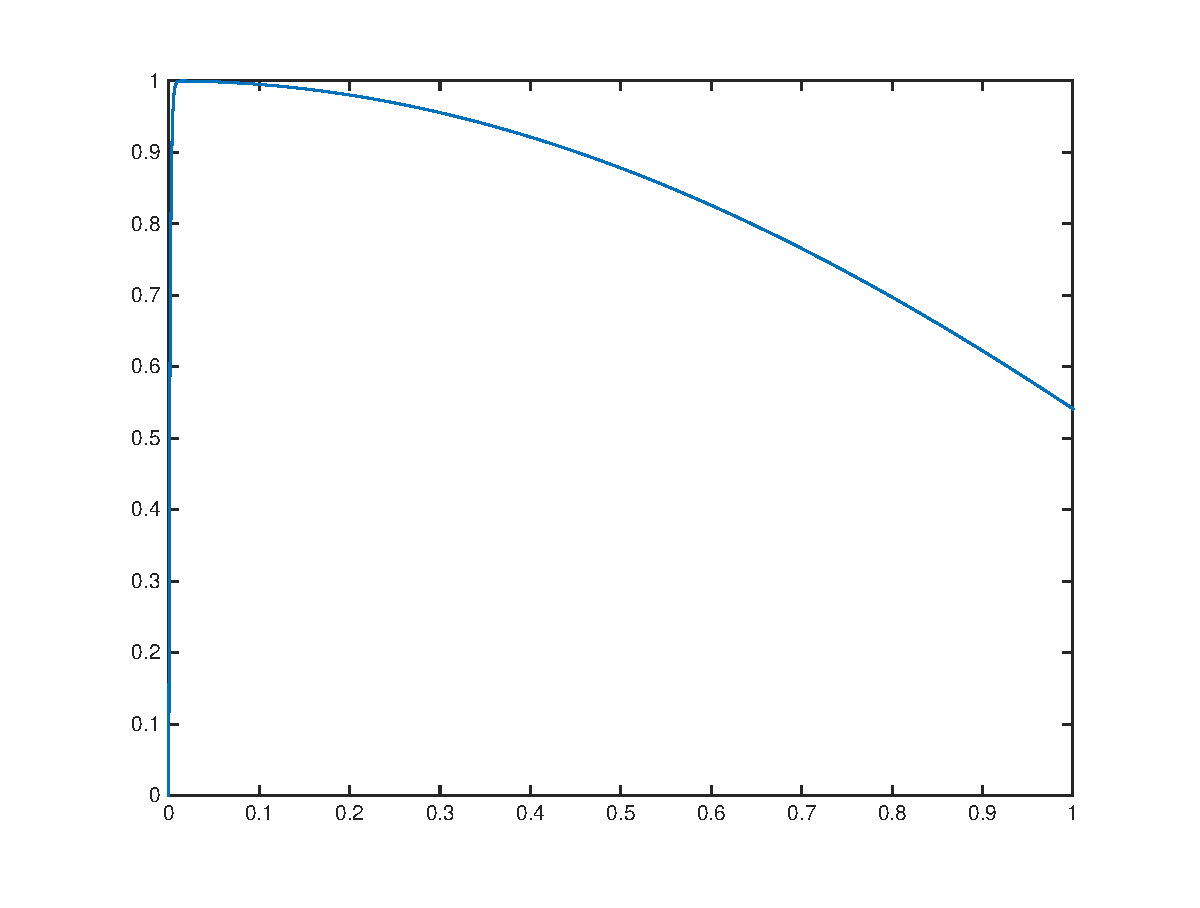
\includegraphics[width=5.5in]{Gear0.eps}}


\item  \(u_0=1\)时,Gear方法如图

\centerline{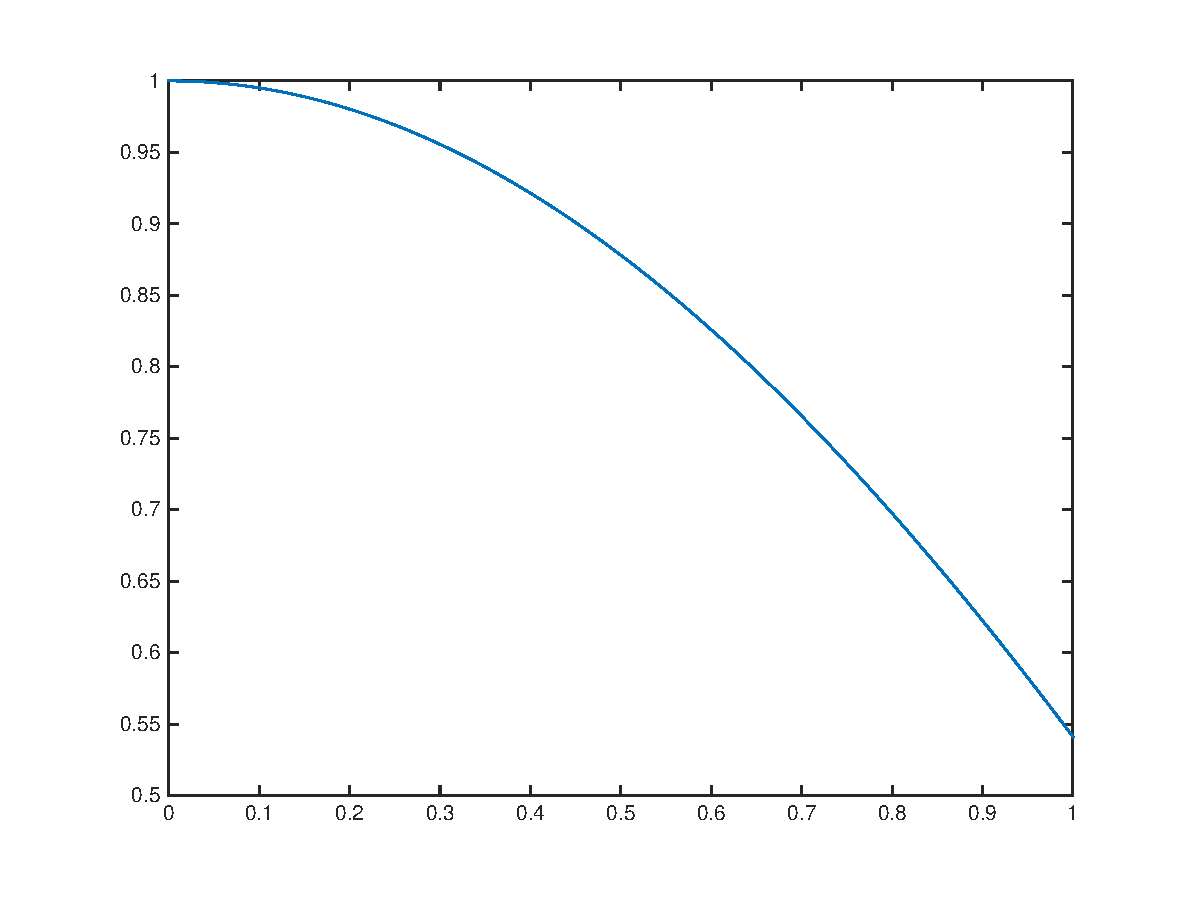
\includegraphics[width=5.5in]{Gear1.eps}}

\end{enumerate}

当\(\Delta t = 10^{-2}\)时,此时\(\Delta t \lambda = 10\),此时Adamas格式不再稳定:
\begin{enumerate}
\item \(u_0=0\)

\centerline{\includegraphics[width=5.5in]{Adamas01.eps}}

\item \(u_0=1\)

\centerline{\includegraphics[width=5.5in]{Adamas11.eps}}

\end{enumerate}

\end{enumerate}






















\end{enumerate}
\end{document}


















